\chapter{相关工作与预备知识}
\label{cha:2-related}

  与本文研究内容相关的工作主要包括两个方面:黑白图像着色与生成对抗网络。我们将介绍这两个方面的相关工作和本文需要的预备知识。

\section{黑白图像着色}
\label{sec:2-image-color}

  黑白图像着色问题的研究以深度学习的兴起作为分界点分为两个阶段:计算机辅助阶段与计算机全自动阶段,而这两个阶段中的研究重点,研究方法以及效果也是差异很大。

\subsection{计算机辅助的图像着色}
\label{sec:2-user-guided-color}
  
  着色是Wilson Markle在1970年提出的一个术语,用于描述给黑白视频或电视节目添加颜色的计算机辅助的过程。之后这个术语被推广到了所有给单色调图像视频添加颜色的范围。

  最早期的着色完全依赖人工,主要问题在于非常耗时耗力。艺术家要给一张黑白图像着色,先要将它划分为多个区域,然后给每个区域分别指定颜色。分割的过程也可以让计算机自动来做,但分割算法的问题在于无法处理一些复杂的、迷惑的区域边界,比如人的头发和脸。视频的着色还需要追踪区域在帧与帧之间的移动,而现有的追踪算法对于非刚性物体不能稳定追踪。这些问题都会导致人工工作量的增加。

  2003年的一款给静态图片着色的商业软件BlackMagic,给用户提供了有用的画刷和调色板,但分割的任务还是完全由用户完成。

  Welsh~\cite{DBLP:journals/tog/WelshAM02}等人在2002年提出了一种半自动的着色方法,通过将待着色的灰度图像转换成一张给定彩色图像的颜色风格。他们检测灰度图像中每个像素及其领域的灰度值,着色为被参考的彩色图像中灰度对应领域的颜色。效果如图~\ref{fig:transfer}所示。但是这种方法的问题在于对两张图像区域之间的风格相似度要求很高,所以需要一些人工工作量;另外这个方法也没有显式的保证被着色图像颜色的空间连续性。

  \begin{figure}[H]
    \centering
    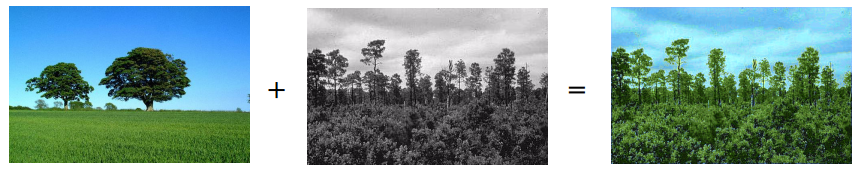
\includegraphics[width=0.7\paperwidth]{transfer_color}
    \caption[Welsh等人的风格转换着色]{Welsh等人的风格转换着色。左边是选择的参考彩色图像,中间是待着色图像,右边是风格转化结果}
    \label{fig:transfer}
  \end{figure}

  Levin~\cite{journals/tog/LevinLW04}等人的方法避开了区域分割的问题,他们做了这样的假设:在时间、空间上连续的并且有着相似灰度的像素应该最终是相似的颜色。在这个假设的基础上,他们设计了一个二次损失函数并将这个问题转换成了一个标准化的最优化问题。他们的输入时认为指定的一些彩色条带,如图~\ref{fig:color_optim}所示,最优化的目标即是在这些已知颜色的像素基础上,最小化相似灰度相邻像素的颜色差。

  \begin{figure}[H]
    \centering
    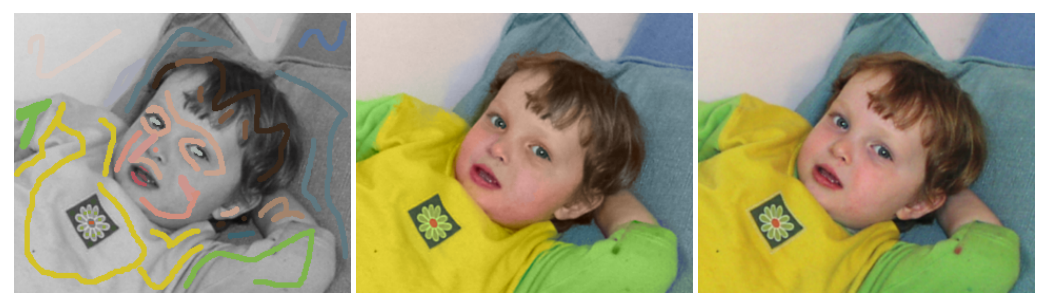
\includegraphics[width=0.7\paperwidth]{color_optim}
    \caption[Levin等人的最优化着色]{Levin等人的最优化着色。左边是人工添加的彩色条带提示,中间是着色结果,右边是原始真实图像}
    \label{fig:color_optim}
  \end{figure}

  不过以上这些计算机辅助着色都有的问题就是需要人工根据经验指定一些区域或像素的颜色,无法完全解放人力。

\subsection{计算机全自动的图像着色}
\label{sec:2-automatic-color}

  随着机器学习与深度学习席卷计算机图像、计算机视觉领域的各个研究方向,也出现了许多关于着色问题的数据驱动方法的研究。

  Cheng~\cite{DBLP:journals/corr/ChengYS16}等人训练了一个神经网络来处理着色。基于学习的着色的基本思路都是:对于数据集中的真实彩色图像,将其变换到LAB或者YUV等个通道、灰度与色度独立的颜色空间,将L空间或者Y空间作为网络输入,而AB或者UV作为真实值,目标就是最小化网络输出与真实值之间的差异。Cheng~\cite{DBLP:journals/corr/ChengYS16}的处理是,对于输入的灰度图像,通过人工设计的特征提取函数得到图像特征,将这个图像特征作为一个包含三个隐含层的神经网络的输入,得到与原图等大的色度图。由于神经网络直接生成的色度图会存在一些不真实点和空间上的颜色不连续性,于是与原始的灰度输入做一个双线性插值得到一个修正后的色度图,然后将灰度图与色度图结合在一起就可以得到着色后的彩色图像。图~\ref{fig:deep_color}就是这篇论文算法的大致流程。

  \begin{figure}[H]
    \centering
    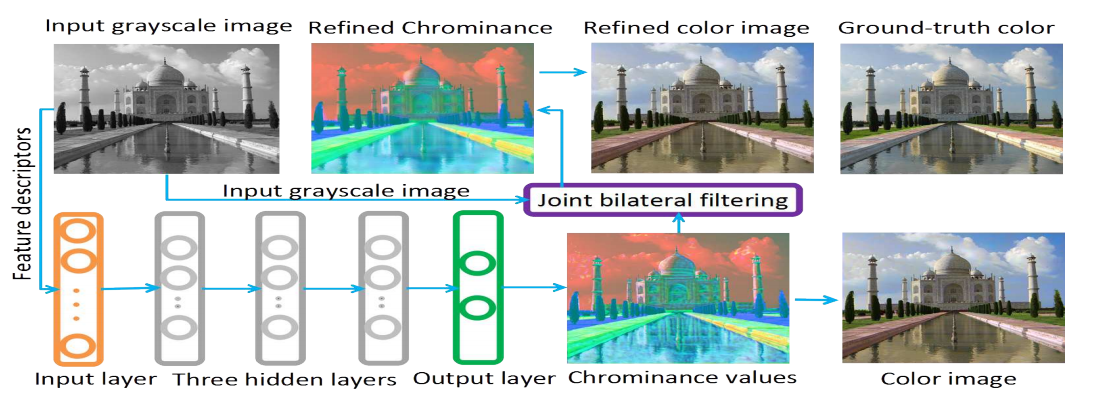
\includegraphics[width=0.7\paperwidth]{deep_color}
    \caption{Cheng等人的算法流程}
    \label{fig:deep_color}
  \end{figure}

  早期神经网络的一个难题就是特征都是人工选取的,特征的效果好坏都需要通过实验说明,而且基于经验的特征选择也是很有限的,只会使用那些经过实验证明可用的特征;另外一点就是能够处理的数据量很有限。Cheng~\cite{DBLP:journals/corr/ChengYS16}的这篇论文也是有很大篇幅在比较各种特征提取函数的效果好坏,图~\ref{fig:feature_choose}给出了他们的一些特征效果的比较。

  \begin{figure}[h]
    \centering
    \subcaptionbox{左图为灰度输入,中间为没有区域特征时的着色,右边是添加了区域特征的结果\label{fig:feature_sub1}}
      {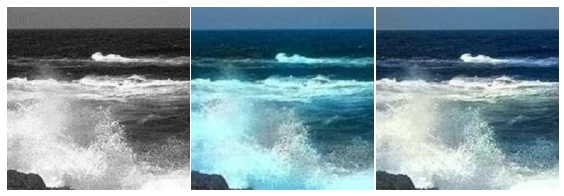
\includegraphics[width=0.3\paperwidth]{feature_sub1}}
    \hspace{4em}
    \subcaptionbox{左图为灰度输入,中间为添加了区域特征和DAISY特征的着色,右边是添加了语义信息特征的着色结果\label{fig:feature_sub2}}
        {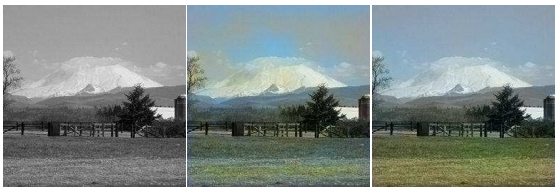
\includegraphics[width=0.3\paperwidth]{feature_sub2}}
    \caption{Cheng论文中的特征选择与比较}
    \label{fig:feature_choose}
  \end{figure}


  CNN的出现就抛弃了人工特征选取的过程,而是一个端到端的训练过程。设计好网络结构以后,以灰度图像直接作为输入,色度图像直接作为输出,经过训练就可以得到直接可用的模型。CNN与ANN在结构上的很大一点不同在于,ANN的相邻两层神经元之间每两个神经元都有信息传递关系,而CNN的相邻两层之间只有空间相邻的神经元才有信息传递,并且同一层的神经元权值共用。这样CNN就可以达到比ANN更深的网络层数和使用更大的数据量,因为它处理的是局部的信息。

  Iizuka~\cite{IizukaSIGGRAPH2016}等人设计了一个更大的CNN网络,并且在更大的数据集ImageNet~\cite{DBLP:journals/ijcv/RussakovskyDSKS15}上进行了训练。他们的核心在于将局部特征与与全局特征进行了结合:局部特征由分辨率较高的卷积层得到,而全局特征由局部特征进一步卷积得到,然后通过一个融合层将局部特征与全局特征结合在一起。得到结合后的特征后,再输入到着色网络,经过一些反卷积层,得到着色结果,最后将着色结果上采样到原图像分辨率结合灰度图就得到彩色图像。图~\ref{fig:let_it_color}即是他们整体的网络结构。

  \begin{figure}[H]
    \centering
    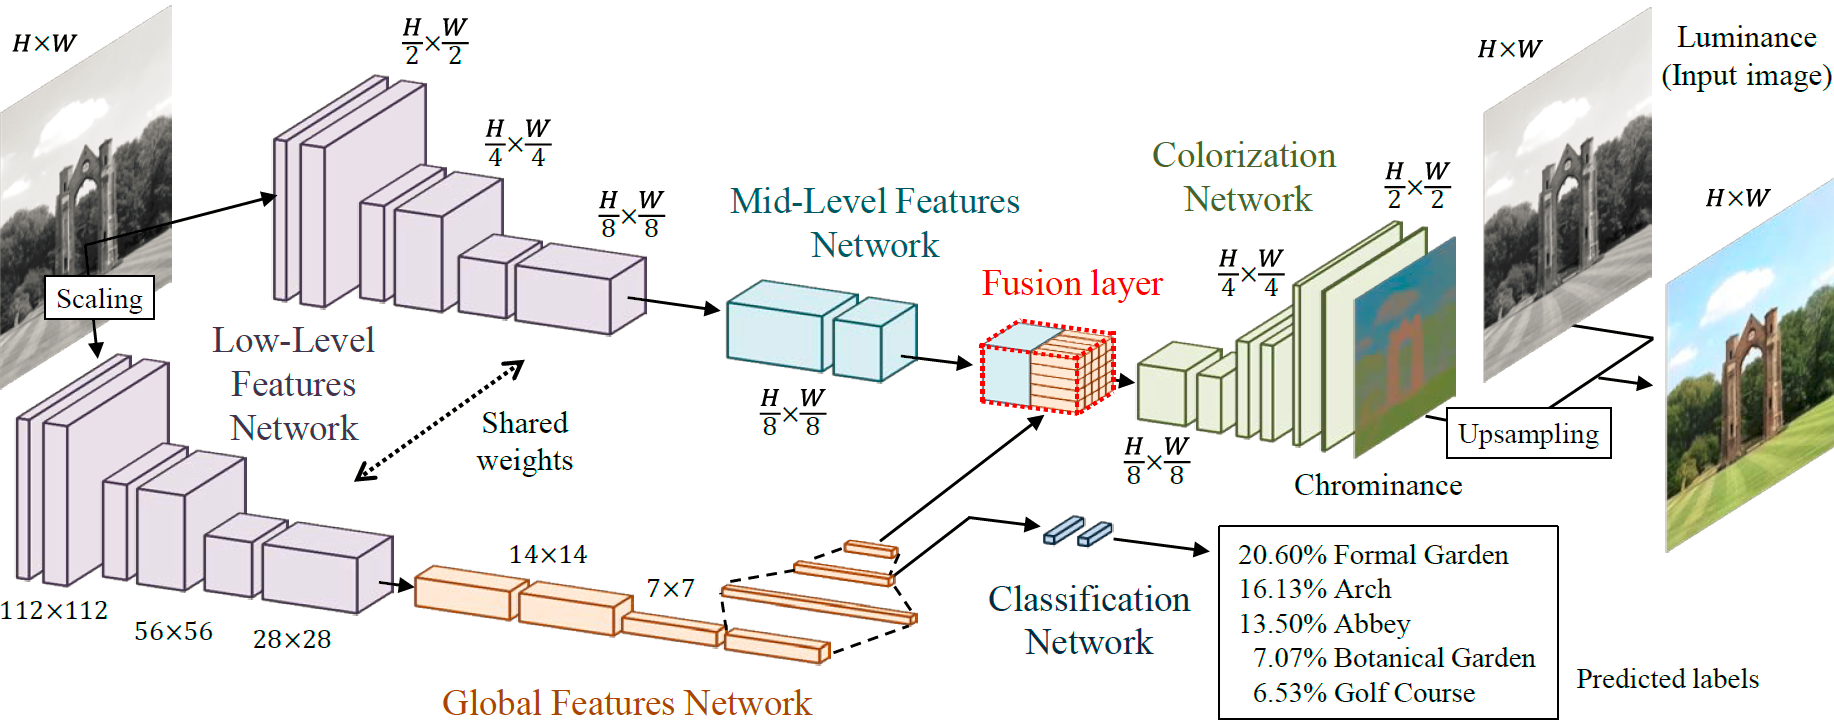
\includegraphics[width=0.7\paperwidth]{let_it_color}
    \caption{Iizuka等人的网络结构}
    \label{fig:let_it_color}
  \end{figure}

  Zhang~\cite{zhang2016colorful}等人从损失函数的角度做了优化。考虑到CNN做着色任务时,对每种物体的着色选择是不一样的,所以网络中会做一些物体识别的判断;而当传统的以欧氏距离作为输出色度图和真实色度之间的损失函数时,对于某个物体的着色而言,使得这个损失在训练集上最小的着色方式,就是将训练集中所有这种物体出现的颜色取平均值,而一个物体往往有许多中可能的颜色取值,比如蓝色的车与红色的车,这样着色的结果就是许多物体最终着色出来都是灰褐色、不真实的结果。所以Zhang~\cite{zhang2016colorful}等人让他们的网络对每个像素输出一个颜色概率分布,然后使用多项交叉熵作为损失函数,这样最终每个像素的着色结果就是在概率分布中取更可能的颜色而不是所有颜色加权平均。另外为了保证像素之间的空间连续性,还要考虑像素之间的联合分布。图~\ref{fig:color_image_color}给出了他们的网络结构。

  \begin{figure}[H]
    \centering
    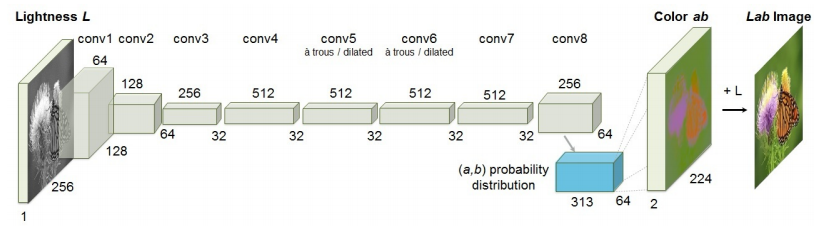
\includegraphics[width=0.7\paperwidth]{color_image_color}
    \caption{Zhang等人的网络结构}
    \label{fig:color_image_color}
  \end{figure}

\section{生成对抗网络}
\label{sec:2-gan}

  生成对抗网络是一种无监督的机器学习模型,最早由Goodfellow~\cite{DBLP:conf/nips/GoodfellowPMXWOCB14}等人在2014年提出,这种模型多用于数据或图像的自动生成,在最近几年里有大量关于GAN的研究,也出现了很多GAN的变体。生成对抗模型的基本结构如图~\ref{fig:gan},其思想为同时训练两个神经网络,一个生成器(generator),一个判别器(discriminator)。输入随机变量到生成器,将期望生成的真实图像与生成器生成的图像混合着输入给判别器,让判别器判断哪些是真实图像哪些是假的图像;通过判别器给出的概率与真实标签的距离更新判别器,同时通过判别器给出的生成器生成图片的真实概率更新生成器。这样两个网络就构成了一种对抗关系,当迭代训练后判别器也难以判断图像的真假,训练好的生成器就可以做图像或数据生成了。

  \begin{figure}[H]
    \centering
    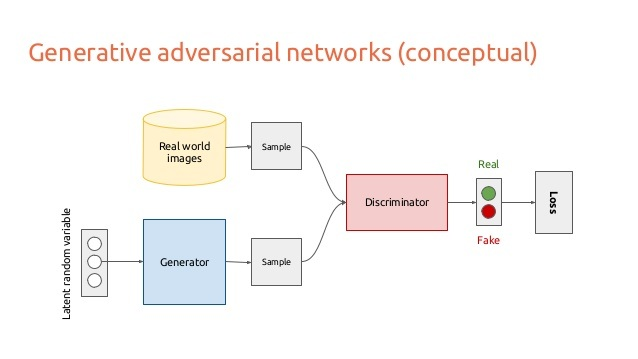
\includegraphics[width=0.7\paperwidth]{gan}
    \caption{生成对抗模型}
    \label{fig:gan}
  \end{figure}

\subsection{cGAN与wGAN}
\label{sec:2-cgan-and-wgan}
  
  GAN模型经过几年的发展出现了许多变体,下面介绍对着色问题有用的带条件的生成对抗网络与沃瑟斯坦生成对抗网络。

  cGAN由Mirza~\cite{DBLP:journals/corr/MirzaO14}等人在2014年提出,基本结构如图~\ref{fig:cgan}。其最重要的一点思想就是当网络需要输入一些额外信息时(例如着色问题中的灰度图像),将这个额外信息同时输入给生成器和判别器,而不是只输入到生成器。实验证明,这样的方式可以让生成器与判别器都收敛得更好。

  \begin{figure}[H]
    \centering
    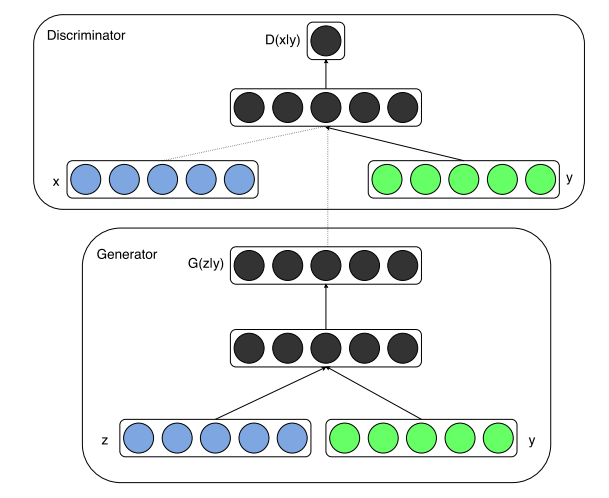
\includegraphics[width=0.7\paperwidth]{cgan}
    \caption[带条件的生成对抗模型]{带条件的生成对抗模型,y即额外信息}
    \label{fig:cgan}
  \end{figure}

  而wGAN的工作则是对原始GAN结构的一些优化,由Arjovsky~\cite{DBLP:journals/corr/ArjovskyCB17}等人2017年提出。我们已经知道GAN是同时训练生成器网络与判别器网络,而且两者的最优化目标是对立的。那么就会有一个平衡二者训练的问题存在:一般情况下,判别器的任务更简单,所以收敛的比生成器就更快,如果判别器早早的就收敛到了很好的状态,生成器怎么更新都无法欺骗判别器,这样生成器的学习就停止了,最后也无法得到好的生成网络。而wGAN就是要解决GAN训练不稳定的问题,他们对原始GAN主要做了4点改动:

  \begin{enumerate}
    \item 判别器最后一层去掉了sigmoid
    \item 生成器以及判别器的损失函数不取对数
    \item 每次更新判别器的参数之后,用一个固定常数将它们的绝对值截断
    \item 不用基于动量的优化算法
  \end{enumerate}

  虽然只是几点小小的改动,Arjovsky~\cite{DBLP:journals/corr/ArjovskyB17}等人在另一篇论文中从数学上证明了这样是可以使GAN稳定训练的,而不需要人工控制生成器与判别器的训练比例。

\subsection{变分自编码器}
\label{sec:2-vae}
  
  对于着色问题而言,我们要通过输入灰色图像得到色度图像输出,而通用的GAN模型中生成器网络的输入是一个噪声向量,所以有必要对生成器网络做一些修改。变分自编码器(VAE)跟GAN一样是非常常用的无监督学习模型,由Kingma~\cite{DBLP:journals/corr/KingmaW13}等人2013年提出。变分自编码器主要由编码器网络与解码器网络组成,如图~\ref{fig:vae}所示,其作用是可以将图片编码为特征向量然后解码出来,为图片变换提供了可能。

  \begin{figure}[H]
    \centering
    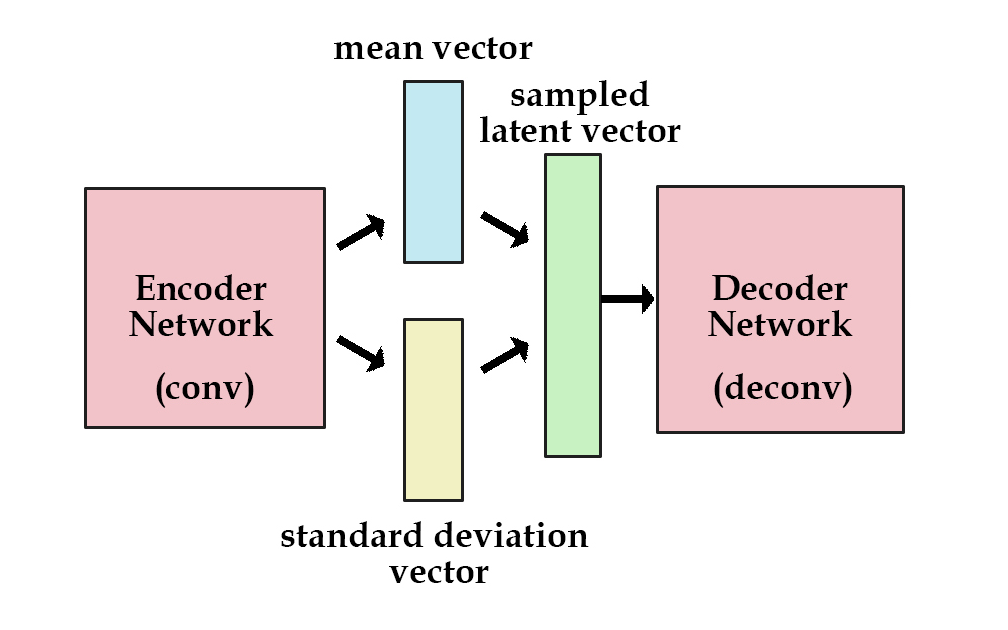
\includegraphics[width=0.7\paperwidth]{vae}
    \caption{变分自编码器}
    \label{fig:vae}
  \end{figure}

